\chapter{Sequential Cognition Processes} \label{chp:scp}
\section{SCPs: An Intuitionist Description} \label{ssec:intu}
\begin{figure*}
\begin{subfigure}{.35\textwidth}
  \centering
  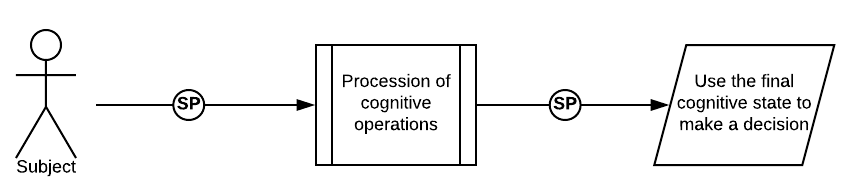
\includegraphics[width=0.97\linewidth]{general}
  \caption{Unrestricted SCP.}
  \label{fig:scp_general}
\end{subfigure}%
\begin{subfigure}{.65\textwidth}
  \centering
  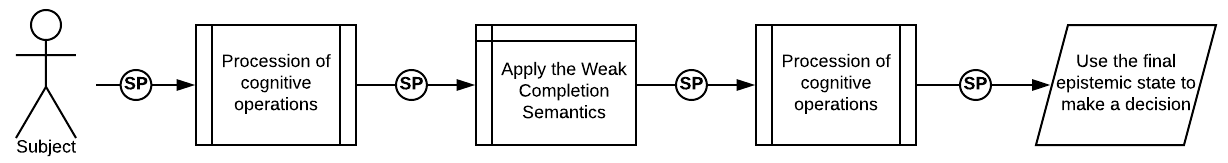
\includegraphics[width=0.97\linewidth]{generalWCS}
  \caption{WCS guaranteed to occur.}
  \label{fig:sfig2}
\end{subfigure}
\caption{The most general description on an SCP with and without guaranteeing the WCS is applied at least once. An agent transitions from one epistemic state to another and then uses it to make a decision. $SP$ nodes indicate state points.}
\label{fig:scp_generalWCS}
\end{figure*}

Although there is evidence that the brain can perform several simultaneous operations when considering a task (such as when considering an image \citep{sigman2008brain}, the SCP framework assumes that at some points in reasoning about a given task, the mental processes of the agent converge to a set of epistemic states, called a \textit{state point}. Whatever happens between these points of convergence can contain any number of parallel processes. The collection of processes that occur between any two state points in a reasoning task is called a \textit{cognitive operation}. It follows that any cognitive operation is valid as long it takes a set of epistemic states as input and produces a set of epistemic states as output. Figure~\ref{fig:scp_general} outlines an SCP-like structure that is powerful enough to model any cognitive task that involves an epistemic state transition. However, it does not provide any useful information; the nature of the processes followed is completely undescribed. Suppose, instead, that some cognitive task is being modelled, and that researchers have reason to believe that The Weak Completion Semantics should play a part in their model. Under this new restriction, and assuming a sufficiently expressive epistemic state, Figure~\ref{fig:scp_general} is still an accurate model of the process, but now so is Figure~\ref{fig:sfig2}. By sacrificing some of the ambiguity -- and, thus, expressiveness -- of the model, the information content of the model description has increased. This trade-off is a feature of the SCP framework and finding the right depth of complexity to model the task accurately and still provide meaningful information is more art than science at present. 

\section{SCPs: Mathematical Formulation}
An SCP Task $\Pi=(s_i, M, f(), \gamma)$ consists of an initial epistemic state $s_i$, a known set of cognitive operations $M$, a desired final output $\gamma$, and an external function $f()$ which generates those final outputs by translating the final epistemic state into an empirically grounded set of possible responses. An epistemic state $s_k$ describes all the information available to the agent at state point $k$. The precise contents of an epistemic state should be chosen so that at least some $m \in M$ are able to accept that state as an input. In the case of a system containing only the one complex operation which applies the WCS, one possible epistemic state is $s=(P,\Delta,V)$, where $P$ is a set of inference rules of the form $(head \leftarrow body)$, $\Delta$ is a set of conditional rules of the form $(\psi|\phi)$ and $V$ is a mapping of atom names appearing in $KB$ to a truth value in \L ukasiewicz logic ($\top,u, \bot$). In principle this definition will serve for the rest of the paper, but it is extended slightly so that $s_k = (S,\Delta,V,R)$ where $R$ is a set of labelled categorization criteria sets (\textit{LCS}). An LCS $ c \in R$ consists of a category name and list of rules and atoms which fit into that category.

A base point is a single epistemic state. A state point $p$ is defined recursively by $p=\{\bar{p} \oplus Q \}$ where $\bar{p}$ is a base point, and $Q$ is a set of state points, and $\oplus$ represents the exclusive-or operation\footnote{$(X \oplus Y) = ((X \cup Y) - (X \cap Y))$ for sets $X$ and $Y$.}. State point containment $\in_s$ for state points $p$ and $q$ is defined recursively as follows:

\[
p \in_s q = \begin{pmatrix} p \in q  & \textrm{True} \\   \exists_{r\in p}p \in_s r = \textrm{True} & \textrm{True}   \\ \textrm{Otherwise} & \textrm{False} \end{pmatrix}
\]

It is never the case that $p \in_s p$.

A cognitive operation $m = (\chi, e), m \in M$ consists of a precondition $\chi$ and a process $e$, such that for an input state point $p$, every base point $\bar{p} \in_s p$ is either accepted as input ($\bar{p} \models m[\chi]$ under whatever definition of $\models$ is used for the complex operation $m$), or else rejected. Every base point is evaluated by the complex operation in isolation (no other base point $\bar{q}$ can affect the output of $m$ on base point $\bar{p}$). To capture the fact that cognitive operation may utilize non-monotonic logic, applying $m$ to an input base point $\bar{p}\in p$ always yields a state point $p'$ (written $J[\bar{p},m]=p'$) which describes all possible resulting epistemic states that can be generated. @TODOextend

Applying $m$ to an input state point $p$ is done by replacing every base point $\bar{p} \in p$ with $J[\bar{p},m]$. A cognitive operation is called monotonic if it always yields a base point as an output given a base point input ($J[\bar{p},m]=\bar{p'}$). It follows that the depth of a state point is directly related to the number of complex operations which have been performed in the SCP prior to its occurrence. If a base point does not meet the precondition, it is either ignored completely and not processed (\textit{cruel application}), or passed exactly as is to the next complex operation (\textit{lenient application}). It is worth noting that the type of cognitive states produced as output by $m$ may not be the same as those of the input.

This paper will focus on cases where the type of cognitive state remains constant, but there is no reason in principle that a base point input $s_k = (P,\Delta,V)$ for the WCS could not be returned as a base point $s_k = (P,\Delta,V,R)$ where $R$ is a categorization variable (Section~@TODOref). Future models of human cognition may well rely on background knowledge which draws inferences from multiple types of non-monotonic logics.

An SCP $(\pi,f())$, $\pi=(s_i\longmapsto m_1\longmapsto ...\longmapsto m_n)$ describes an initial epistemic state (or state point if the input is uncertain) and state point $p_k$ is defined recursively by $p_k = J[p_{k-1},m_k]$. An SCP is called \textit{credulously valid} if $f(p_n) \models \gamma$ for at least one epistemic state in the final state $p_n$. An SCP is called \textit{sceptically valid} if $f(p_n) \models \gamma$ for every epistemic state in the final state. In cases where all operations are monotonic, sceptical validity is the same as credulous validity.

Finally, a \textit{realised SCP} $r = (\mu, f())$ where $\mu=K[\pi]$, and $K[\pi]=s_i \longmapsto (m_1,\bar{p}_1) \longmapsto ... \longmapsto (m_n,\bar{p}_n))$ where, for every pair $(m_i,\bar{p}_i)$, $\bar{p}_i \in J[\bar{p}_{i-1},m_i]$. Realised SCPs describe a single agent's interpretation of an SCP and associate only a single epistemic state, rather than a state point to the output each cognitive operation in an SCP. 

When every cognitive operation in $M$ is monotonic, it is trivially easy to transform and SCP into a realised SCP and vice versa @TODOproof. In cases where SCPs are monotonic, we will use the SCP and its realised SCP interchangeably. The number of realised SCPs for an SCP is the same as the number of base points in the final state point of that SCP.



\section{SCP Tasks vs. SCPs vs. Realised SCPs}

SCP tasks describe a problem that needs to be solved and the limitations which the solution must to adhere to; SCPs describe a single 'recipe' that can be used to describe a sequence of well-founded, non-monotonic operations which an agent might use to model a problem; and realised SCPs describe how adherence to specific SCP can result in some agent coming to a conclusion that matches empirical data.

For a given SCP task there can be many possible SCPs (the question of how to choose the most probable of these candidate SCPs is discussed in Section~@TODOref), or no possible SCPs at all.

Figure~\ref{fig:scpExam} illustrates a situation in which students are asked if they will pass their next exam, and considers the example from the perspective of the SCPs task and associated variables, two possible SCPs describing different approaches to modelling the Task, and the Realised SCPs which could result. This figure is provided using propositional logic, and examples using non-monotonic logic will be introduced in Section~\ref{chp:experiments}.

\begin{figure}
\begin{center}
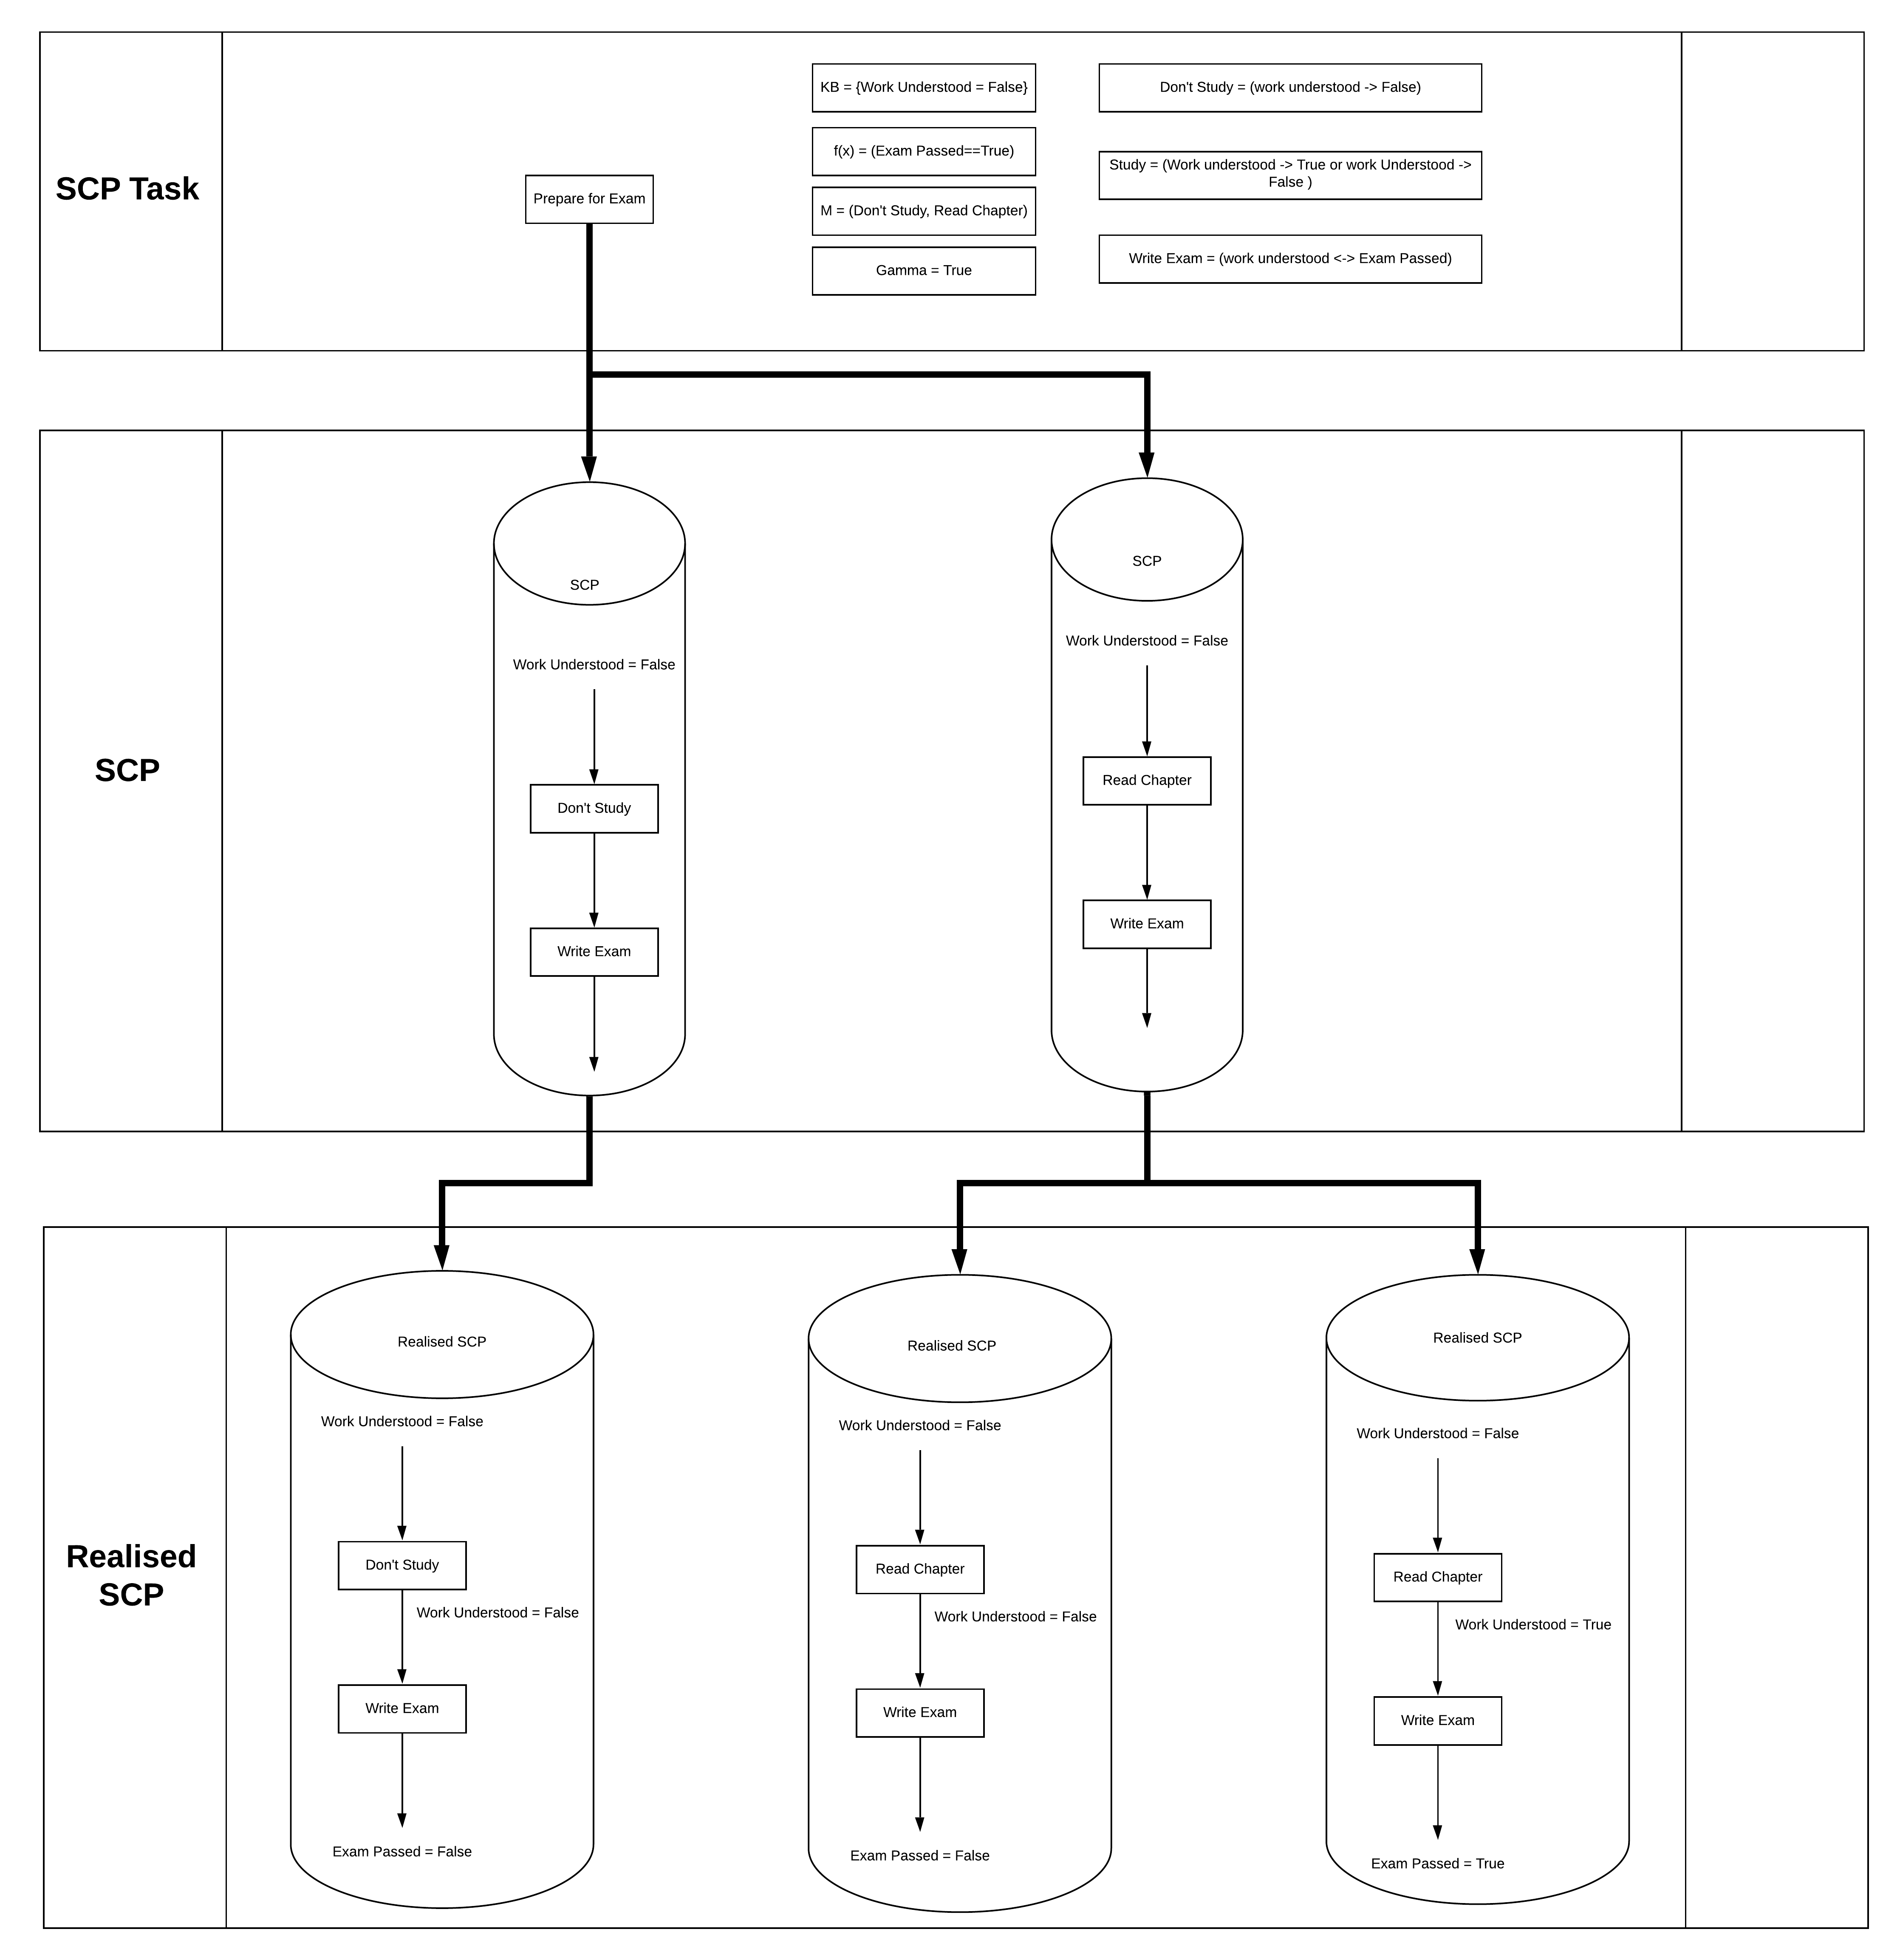
\includegraphics[scale=0.4]{ExamSCP}
\end{center}
\caption{An SCP Task, SCP, and Realised SCP describing whether a student will pass their exam. @TODOredodiagram}
\label{fig:scpExam}
\end{figure}

\section{Epistemic States}
The choice of epistemic state is dependent on the properties that are known or suspected to be true for the cognitive task as a whole. For example, a researcher working on drawing inferences using Propositional Logic can be certain that any SCP they create should be expressive enough to pass a knowledge base to a cognitive operation. Thus, it might suffice to simply define $s_i=(KB)$ where $KB$ is a set of propositional rules. By contrast, a researcher using the WCS requires a system capable of both communicating a set of rules to the next complex operation, and of describing the results of repeated applications of the semantic operator. It might seem intuitive to simply append a set of conditional rules $\Delta$ to the state used for the propositional case and to use a the semantic operator as an external function to evaluate the SCP. And, though this approach works for many examples, it makes it impossible to perform further processing in the SCP \textit{after} applying the semantic operator. What if the conclusion drawn was meant to form part of the background knowledge of another process? In practice using $s_k=(S,\Delta,V, R)$, where $V$ is a set of (variable name, value pairs) and $R$ is a categorization variable, seems able to model all aspects of the WCS, including information related to the least model. 

As yet, there are no definite rules for creating an epistemic state, but Albert Einstein's famous advice from 1950 still rings true: ``Everything should be made as simple as possible, but no simpler.'' The ideal epistemic state is one that enables every reasonable cognitive operation in $M$ that might help model the problem, without adding superfluous functionality that might render searching the SCP space infeasible.

\subsection{State Points}

\subsection{The Categorization Variable}
%@TODOreformulatefors_k=(s,v,delta,r)
The final property of a cognitive operation that needs to be discussed is how it is able to interact with the categorization variable $R$. Imagine a case drawn from \cite{saldanha2017weak} where the difference between creating abnormalities for obligate and factual conditionals is discussed. The intuition behind the authors' work can be summarised by saying that there are two different types of conditional statement, those that \textit{have to be} true, and those that are \textit{usually} true. If it rains $r$, I will normally take my umbrella $u$ (in the absence of something abnormal happening, like a plague of umbrella-stealing gnomes). This a statement that is usually true, but some things are definitely true. For example, when it rains, water has to fall out of the sky $s$. This is an essential property of rain, not subject to abnormalities. Thus one useful set of categorizations for researchers seeking cosmic knowledge of weather patterns may be: $R=\{obligate: \{u \leftarrow r\}, factual: \{s \leftarrow r\} \}$. With these labels we might then expect that the process followed by the operation $m \in M$ which creates abnormalities would treat the two conditionals in $KB$ differently, because of their assignments in $R$. $R$ then is a way of expressing meta information to the cognitive operations, and it is completely possible that some operation $m_k$ might change $R$ is such a way that future operation $m_{k+l}$ produces different output. This is a technique we will exploit in several examples in this paper.

@TODOdefinereachability
\section{Cognitive Operations}
The set of possible complex operations $M$ determines many attributes of the achievable final state point $p_n$. If every $m \in M$ is monotonic, then $p_n$ will be monotonic. If some cognitive operation is computationally complex or produces a very large number of output state points, then search using that base point becomes less efficient. If some complex operation $m'$ (such as weakly completing) is known or believed to occur in the SCP, then a restriction on the cognitive states exists such that either the initial state is of a format suitable as input for $m'$, or there exists another cognitive operation which is able to output a state point which contains base points of a suitable format.

More abstractly, the set of cognitive operations should be well-founded in the literature. The set of possible complex operations is infinite and an SCP only meaningfully describes human cognition when it contains cognitive operations that have been justified empirically (\textit{modus ponens-modus tolens} asymmetry, suppression, denial of the antecedent, etc.). 

\subsection{Pre-conditions and Effects} \label{ssec:precond}
The precondition $\chi$ of a cognitive operation $A$ refer to those conditions the input state point must satisfy in order for that operation to be considered valid. An SCP is valid if and only if every cognitive operation it contains is valid. For example, one might have a cognitive process describing Julie's plans for a night out on the town. Let us imagine that the SCP task describing her night out includes the operation \texttt{goHomeByCar}. Semantically, this operation should take her \textit{isHome} variable and set it to True.

The situations in which \texttt{goHomeByCar} can reasonably occur in an SCP are at the researchers' discretion. Researcher~1 might feel that it can be allowed at any point in the SCP and will simply have no effect for those input epistemic states in which she is already at home. Researcher~2 might argue that \texttt{goHomeByCar} is applicable only when \textit{isHome}=False. Researcher~3 knows that only the cognitive operation \texttt{goToClub} changes the \textit{isHome} variable, and so argues that \textit{isHome} is only applicable after \texttt{goToClub} occurs. There are merits to the arguments of each researcher.

Researcher~1 argues for a property called \textit{trivial validity}, that is that SCPs should always be considered valid, without any need for evaluation. This approach, however has one significant drawback: it cannot handle changes in the structure of epistemic state inputs. Imagine an epistemic operation called \texttt{dontDriveDrunk} which corresponds to our party animal realising that she shouldn't drive home of she's been drinking. Imagine further that this operation takes base points which are either of propositional or default structure (@TODOrefsection) and outputs an epistemic state of default structure which contains the new rule. If \texttt{goHomeByCar} took only a propositional state as input, then any sequence where \texttt{dontDriveDrunk} occurs as the previous operation will cause the SCP to fail because of the input state is not of an allowed type. Trivial validity then, is not sufficient for modelling SCP which state structure changes.

Researcher~2 has opted for a \textit{variable validity} approach. She has reasoned, correctly, that the \texttt{goHomeByCar} only results in an epistemic state change when when \textit{isHome} is not True. She therefore, feels that it only makes sense to reduce redundancy and search complexity in creating the SCP by only allowing the action to occur when it can be said to have an effect. This argument has some merit from an intuitive perspective, but presents an unpleasant question: what if there are state points in which only some ground points actually meet the precondition? To compound the troubles with this variable state approach to preconditions is the fact that it is not possible to determine SCP validity without evaluating the SCP at runtime, which could be slow for large SCPs.

Researcher~3 has taken an \textit{operator validity} approach, instead has focused on the structure of the SCP. This approach allows SCP validity to be determined without explicitly evaluating an SCP, one need simply search through the cognitive operations in the SCP to make sure that no operation has a precondition operation which has not yet occurred. This approach also presents drawbacks, it requires explicit knowledge of operation interactions, and adding a new cognitive operation to $M$ in the SCP Task might force several other operations to update or change their interactions. Further, there might be other cognitive operations which mean that the precondition operation is no longer in effect. Imagine a third operation \texttt{goHomeByTrain} which also sets \textit{isHome} to True. Now the sequence of operations $x\longmapsto \texttt{goToClub} \longmapsto \texttt{goHomeByTrain} \longmapsto \texttt{goHomeByCar}$ would still be valid with Researcher 2's original requirement that  \texttt{goToClub} occurred previously in SCP. However, it is obvious that \texttt{goHomeByTrain} has negated the effect of \texttt{goToClub}. Evidently this approach is not appropriate in any case in which other operations can silence the effect of those operations mentioned in preconditions.

Every approach has shows strengths and weaknesses, a final approach to consider is the \textit{hybrid validity} approach. With this approach, all cognitive operations are assumed to be valid, provided that the output base points of the previous operation are of a suitable input type for the current operation. Hybrid validity is an appropriate approach for all SCPs in which every cognitive operation has a known output structure. Though hybrid validity does not have the best-case search properties of the other approached, its universal validity means that it should generally be the starting point for generating SCPs. The hybrid approach is followed implicitly throughout the rest of this thesis and preconditions are omitted.

\subsection{Optimality, Satisfaction, Validity} \label{ssec:validity}
\subsubsection{Validity}
As discussed in Section~\ref{ssec:precond} validity can be defined for a cognitive operation and its input. Reaslied SCPs describe both the operation and the input for an SCP and allow us to define SCP validity as follows:

%generated from SCP $(\pi=(s_i \longmapsto m_1 \longmapsto ... \longmapsto m_n), f())$ was in here
A realised SCP $r=(k \in K[\pi],f())$, $k=(s_i \longmapsto (m_1,s_1) \longmapsto ... \longmapsto (m_n,s_n))$ with evaluation function $f()$ is valid iff $s_i$ is an epistemic state, every $m \in \pi$ is valid (according the validity requirements defined by the researcher), and $f(k)$ is defined. 

@TODOredefineKinFirstappearance

An SCP $(\pi,f())$ is valid if and only if there exists some realised SCP $r=(k \in K[\pi],f())$ which is valid.

An SCP Task $\Pi=(s+i, M, \gamma, f())$ is valid if and only if there exists some SCP $((\pi,f())$, with $(\pi=(s_i \longmapsto m_1 \in M \longmapsto ... \longmapsto m_n \in M)$ which is valid.

Validity does not require that $f(\pi)=\gamma$, only that external function $f()$ is able to make some prediction or set of predictions based $\pi$.


\subsubsection{Satisfaction} 

%generated from SCP $(\pi=(s_i \longmapsto m_1 \longmapsto ... \longmapsto m_n), f())$ was in here
A realised SCP $r=(k \in K[\pi],f())$, $k=(s_i \longmapsto (m_1,s_1) \longmapsto ... \longmapsto (m_n,s_n))$ with evaluation function $f()$ satisfies goal condition $\gamma$, written $r\models \gamma$ if and only if $r$ is valid, and $f(k)\models \gamma$. 

An SCP $(\pi,f())$ is satisfies $\gamma$, written $(\pi,f())\models \gamma$, if and only if there exists some realised SCP $r=(k \in K[\pi],f())$ for which $f(k)\models \gamma$.

An SCP Task $\Pi=(s+i, M, \gamma, f())$ is satisfies $\gamma$, written $\Pi\models \gamma$, if and only if there exists some SCP $((\pi,f())$, with $(\pi=(s_i \longmapsto m_1 \in M \longmapsto ... \longmapsto m_n \in M)$ which satisfies $\gamma$.

Heuristic Searches and machine learning techniques are generally used to find satisfying solutions for situations in which it is possible for an answer to be good enough for practical purposes. 

\subsubsection{Optimality}
Optimality refers to finding the best possible SCP to describe a problem according to whatever criteria are used to evaluate the SCP (Section~\ref{ssec:limCogOp}). Loop-free SCPs are candidates for exhaustive search techniques to find optimality, but in practice, loop free SCPs can seldom be guaranteed when there are many cognitive operations in $M$ @TODOproof?. As with all exhaustive search techniques, optimality can be guaranteed for searches of restricted depth even when SCP space contains infinite loops.

%generated from SCP $(\pi=(s_i \longmapsto m_1 \longmapsto ... \longmapsto m_n), f())$ was in here
A realised SCP $r=(k \in K[\pi],f())$, $k=(s_i \longmapsto (m_1,s_1) \longmapsto ... \longmapsto (m_n,s_n))$ generated from SCP $(\pi=(s_i \longmapsto m_1 \longmapsto ... \longmapsto m_n)$ with evaluation function $f()$ is optimal for goal condition $\gamma$ and heuristic function $g()$, written @TODO, if and only if $r\models\gamma$, and $\forall r'=(k' \in [K[\pi]], f()), g(r)\geq g(r')$. 

An SCP $(\pi,f())$ generated from  $\Pi=(s+i, M, \gamma, f())$ is is optimal for goal condition $\gamma$ and heuristic function $g()$, written @TODO, if and only if $(\pi,f()) \models \gamma$ and there exists no other $\gamma$ - satisfying SCP $(\pi,f())$ which can be generated from $\Pi$ for which $g(\pi')>g(\pi)$.

Optimality is not defined for SCP Tasks.






Formally, an SCP $\pi=(\pi_0 \longmapsto ... \longmapsto \pi_n)$ generated from SCP Task $\Pi=(s_i, M, \gamma, f())$ with evaluation function $h()$ is optimality iff $f(\pi)$ is satisfying and there exists no SCP $\pi'$ such that $g(\pi)<g(\pi')$.

In an SCP context a solution may be optimal for a given task or set of empirical data, but only globally valid or satisfying. A significant part of the appeal of the SCP framework is the potential to use high-scoring local solutions to several tasks or from several reasoners and to predict which are most likely by searching for evidence of repeated structures in the disparate solutions.

\begin{table}
\begin{center}
\begin{tabular}{ M L L L}
 \textbf{Validity} & \textbf{Full SCP evaluation} & \textbf{Uniform Epistemic Structure} & \textbf{Operator Silencing Knowledge}\\ 
 Trivial & \text{\sffamily X} & \checkmark & \text{\sffamily X} \\ 
 Variable & \checkmark & \text{\sffamily X} & \text{\sffamily X} \\ 
 Operator & \text{\sffamily X} & \text{\sffamily X} & \checkmark \\ 
 Hybrid & \text{\sffamily X} & \text{\sffamily X} & \text{\sffamily X}
\end{tabular}
\caption{SCP property requirements for precondition types in cognitive operations.}
\label{tbl:solutionSpace}

\end{center}
\end{table}



\section{External Evaluation Functions}
The external evaluation function $f()$ is responsible for evaluating the final state of the generated SCP to map it to the observed or predicted empirical data observed in respondents. The $f()$ function in general is an unbounded tool for making a decision with an epistemic state.

As a function, defining $f()$ forces researchers to specify what information in the epistemic state corresponds to empirical data. The exact procedure by which $f()$ makes this decision should correspond to researcher's chosen criteria for decision making.

For example, in the Suppression task, as formulated in Section~@TODOref, one could define an external activation function $f_{sup}()$ with an output domain of $\{\textrm{She will study late in the library}$, $\textrm{She will not study late in the library}$, $\textrm{Uncertain}\}$. The function must output one of these two responses, regardless of the epistemic state it is given to evaluate. And, when using the WCS formulation of the task, $f_{sup}()$ might be defined as follows:
\[
f_{sup}(s_n) = \begin{pmatrix} s_n \models l\in kb \land l=\top& \textrm{She will study late in the library} \\  s_n \models l \in kb \land l=\bot  & \textrm{She will not study late in the library}   \\ \textrm{Else} & \textrm{Uncertain} \end{pmatrix}
\].

The question of how to select the right external evaluation function is not a focus of this thesis, but, where necessary, all used evaluation functions will be justified with respect to either common-sense reasoning, or evidence that such a function is already used in a more informal way in the existing literature for that experiment.

In general an external activation function is applied to an SCP or realised SCP, but there is no reason one could not be applied to an SCP task as a whole.

The desired final output $\gamma$ simply specifies which output of $f()$ corresponds with observed empirical data of the task under examination. If an SCP is being generated for a task without a known output, $\gamma$ is set to the entire domain of $f()$ so that every response is accepted.

\section{Search in SCP-Space}
As with any data structure in which one input can produce one or multiple outputs, it is possible to search through SCP space in order to find those SCPs which meet certain criteria. Those criteria might be \textit{validity} (Section~\ref{ssec:precond}), \textit{satisfaction} (conditions in $\gamma$ are satisfied), or \textit{optimality} (there exists no better solution to this problem).

SCPs lend themselves particularly well to forward search techniques (@TODOref) but also have some potential using backwards or biderectional search (@TODORef, @TODOref). 

Searching through solutions to an SCP task takes one of two forms \textit{De Novo search}, and \textit{Insertion search}. De Novo search generates an SCP that meets the optimality, satisfaction, or validity requirements of the researcher from scratch, using only the information contained in the planning task. Insertion Search changes an existing SCP which models a particular response in order to model a reasoner with differing responses. Section~\ref{ssec:denovo} and Section~\ref{ssec:insertion} discuss the philosophy, applications and mechanical considerations of these two search approaches.





\subsection{De-Novo SCP Searching} \label{ssec:denovo}
De Novo (from new) search is a search technique in which a final desirable world state is achieved by generating a sequence of actions from a known initial state. An SCP Task contains all the information required to conduct a de Novo search through the space of allowable SCPs for a given cognitive task. The exact search techniques used can be easily varied, but we will consider de Novo search in terms of a breadth-first traversal (@TODORef). 

Figure~\ref{fig:deNovo} illustrates the process by which breadth first search over an SCP task $\Pi=(x,M,\gamma,f())$ can be conducted. Search terminates if a structural inconsistency between two states in $\pi=(x\longmapsto A_0 \longmapsto ... \longmapsto A_n)$ occurs (e.g. output state point structure of $A_k$ does not match expected input structure of $A_{k+1}$). Operator sequences are added to the list of solutions if and only if they meet the validity requirements of the search being used, as discussed in Section~\ref{ssec:validity}. 

In practice it becomes necessary to limit the search depth of the algorithm to search tractable in most cases, and in some cases, search space and solution space may both be infinitly large, as suggested by Proof~\ref{proof:infiniteSCPLength}.

\begin{figure}
\begin{center}
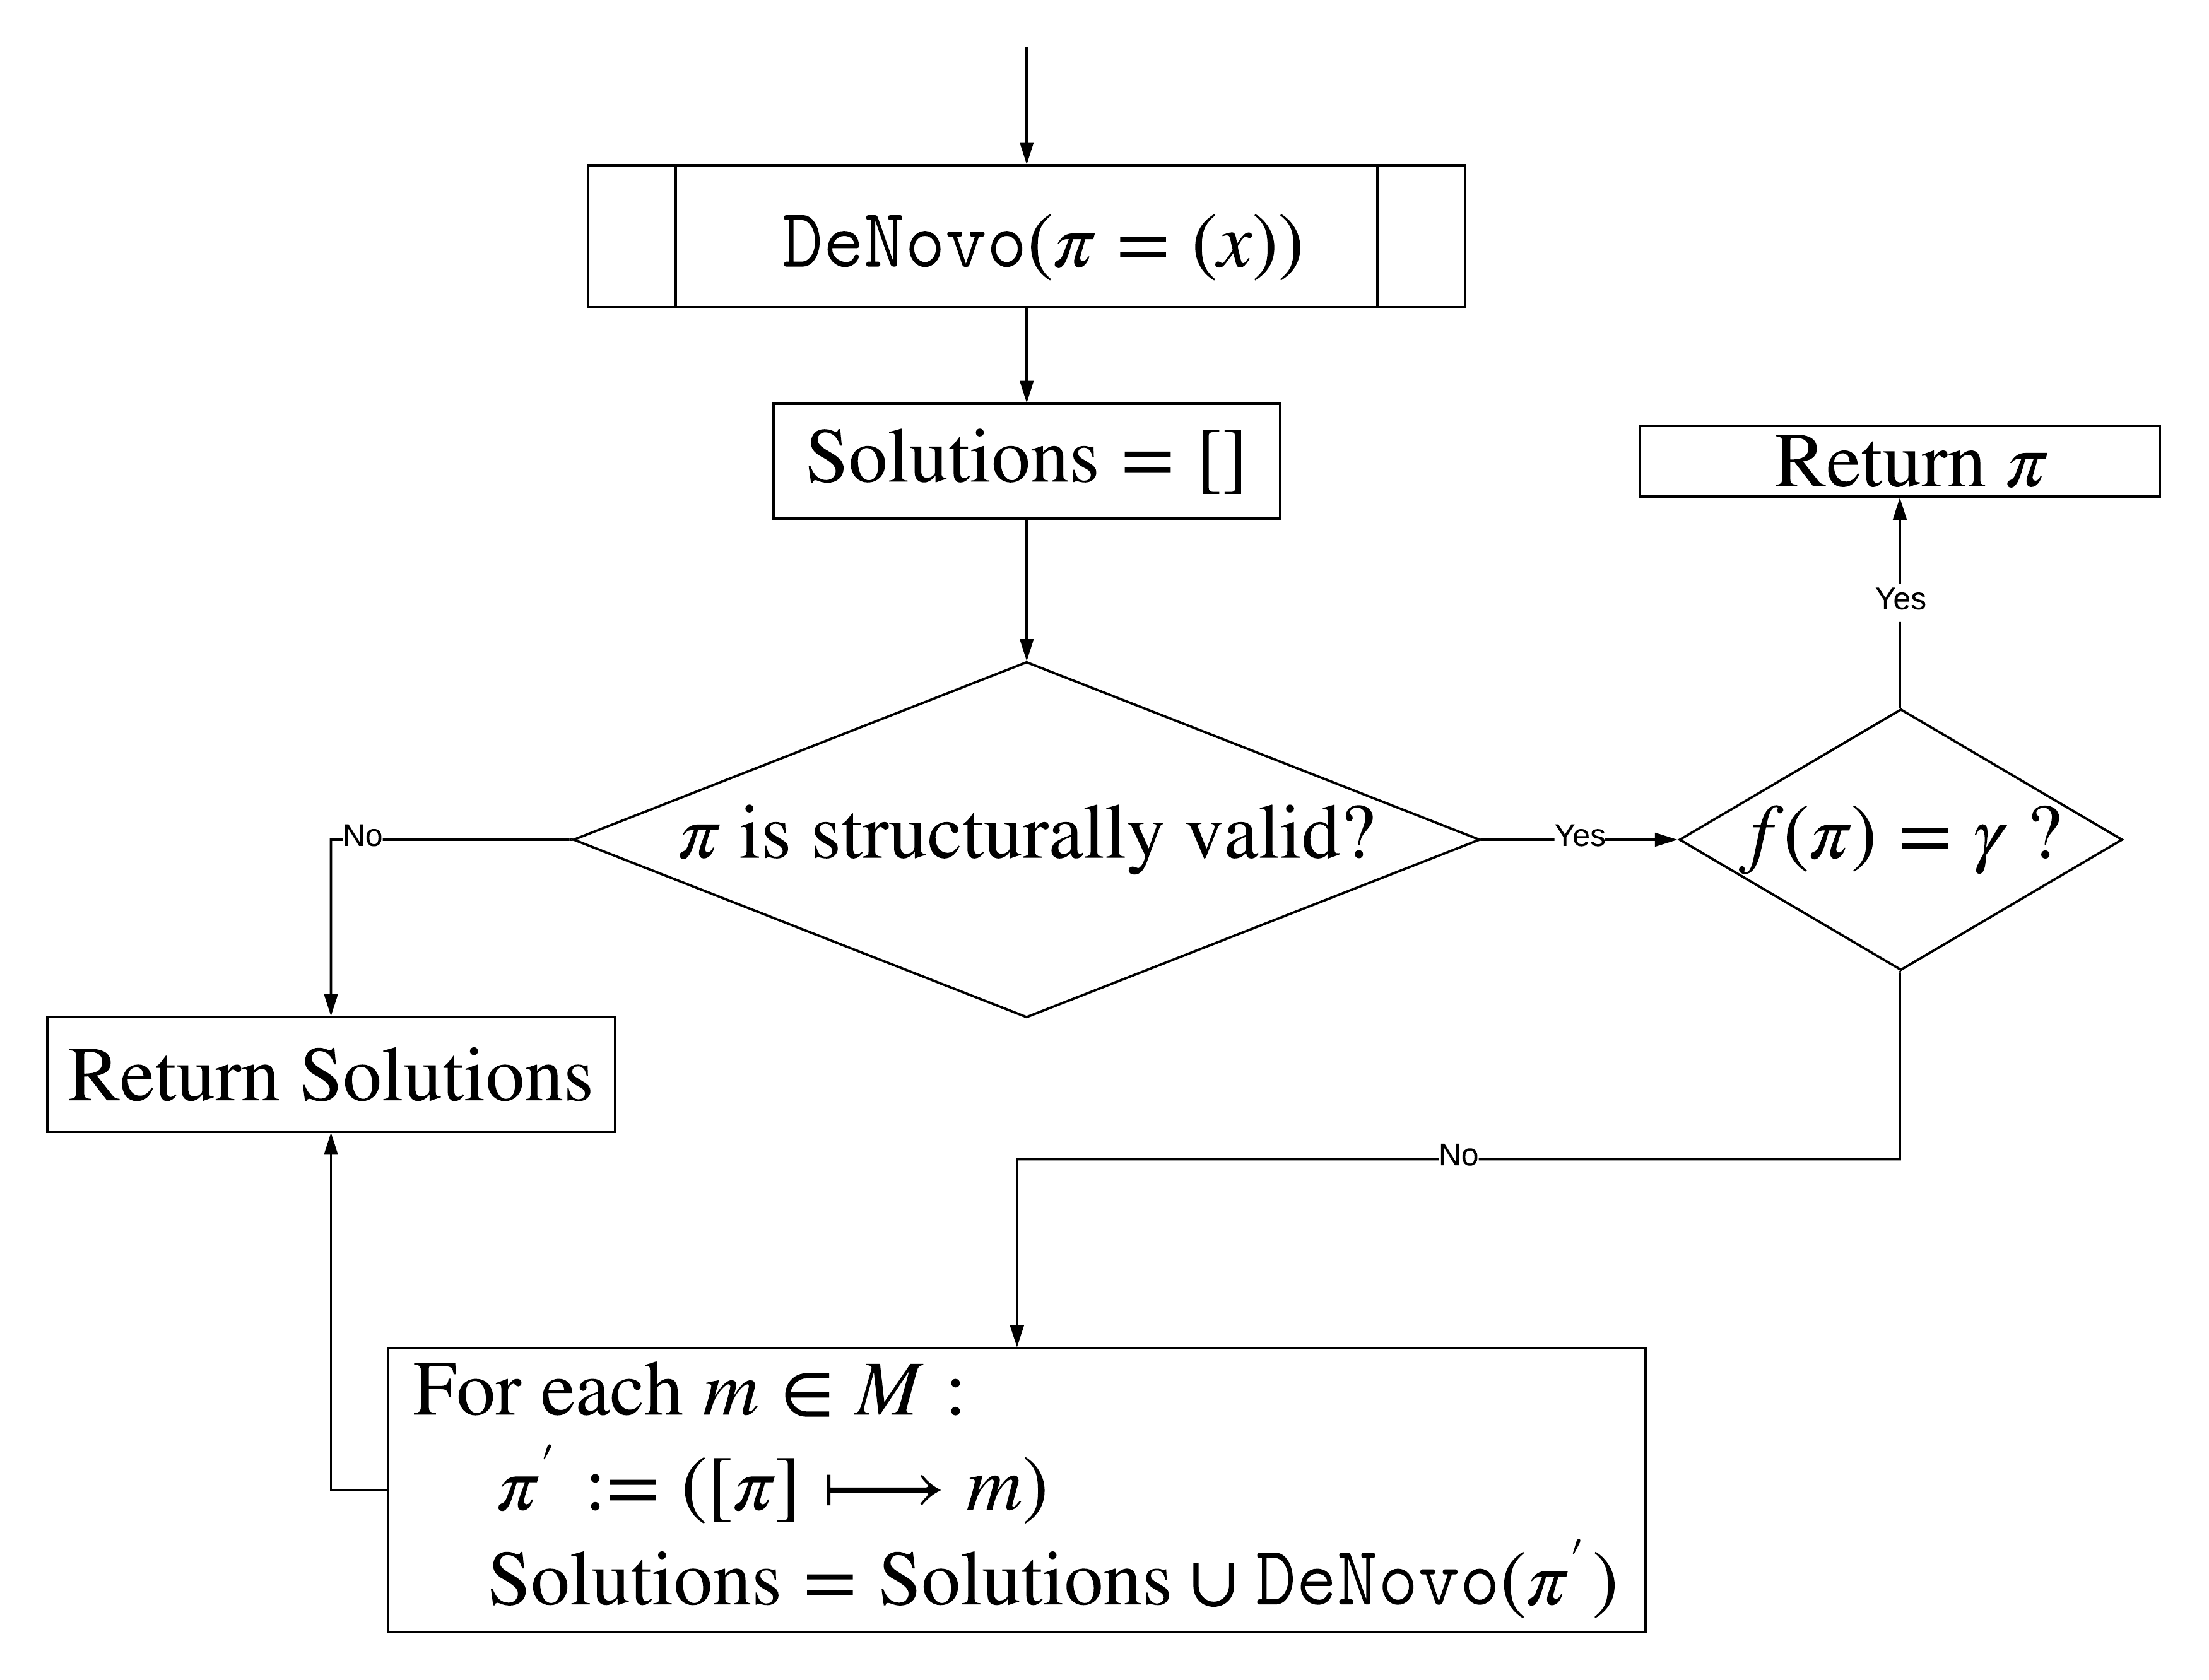
\includegraphics[scale=0.4]{deNovo}
\end{center}
\caption{A breadth-first search algorithm for De Novo SCP search with SCP Task $\Pi=(x,M,\gamma,f())$.}
\label{fig:deNovo}
\end{figure}

\subsection{Insertion Search}\label{ssec:insertion}

Changing the structure of an existing SCP allows researchers to model deviations from standard reasoning for a task. For example, in Section~@TODOref we show that slight modifications to an SCP that models the standard case of the suppression task can lead to an SCP which is able to model reasoners who achieve that classical valid conclusion that she will study late in the library.

The insertion search modifies an existing SCP:
\[\pi=\{s_i \longmapsto A_0 \longmapsto ... \longmapsto A_n\}\]

to produce a new SCP:

\[
\pi'=\{s_i \longmapsto B^*_0 \longmapsto A_0 \longmapsto \longmapsto B^*_1... \longmapsto  B^*_n \longmapsto A_n \longmapsto  B^*_{n+1}\}
\] 

Where $B^*_i = (B_0\longmapsto ...\longmapsto B_n)$, $B \in M$  or is the trivial operation $T$ which returns input state point as output. When describing the SCP, $T$ operations are generally omitted.

In general, Insertion Search is a more difficult search type than De-Novo Search (which is equivalent to an Insertion Search in which the initial SCP is empty). The reason for this is that it is possible for a single insertion to result in an invalid SCP, but adding additional cognitive states may revalidate the SCP (Proof~\ref{proof:insertionSearch}).

This consideration means that it is potentially necessary to insert an unbounded number of new cognitive operations at each point in $\pi$ to find those insertions which are valid. When the total number of new cognitive operations to insert is bounded by $N$, however, it becomes possible to generate every possible subsequence of operation insertions of length $\geq N-k$, where $k$ is the number of insertions already used in the search, for each position $B^*_i$ and determine for which of the resulting SCP cognitive operations sequences $f(\pi')$ is valid.

Figure~@TODOfigure illustrates the process of bounded breadth-first search for Insertion Search.

\begin{proof} \label{proof:insertionSearch}
Given a set of cognitive operations $M$, an external activation function $f()$, and an initially valid SCP $f(\pi)$, $\pi=\{s_i \longmapsto A_0 \longmapsto ... \longmapsto A_n\}$, $A_i \in M$, inserting multiple operations into $\pi$ to create cognitive sequence $\pi'$ may result in a valid SCP $f(\pi')$, when inserting only one operation would result in an invalid SCP.

\begin{itemize}
\item Assume hybrid validity (Section~@TODOsection).
\item Let $f(\pi)=\{True if V is defined\}$, $\gamma = True$.
\item Let $A_x$ be a cognitive operation which transforms an input state point of structure $\{KB, V\}$, where $KB$ contains a set of logical formula of the form $head \leftarrow body$ and every rule in $V$ is of the form $variable \leftarrow value$, where $variable$ is an atom and  $value=\top$ into an output state point of structure $\{KB'\}$, $KB'=(KB \cup V)$.
\item Let $A_y$ be cognitive operation which transforms an input state point of structure $KB'$ into an output state point of structure $\{KB, V\}$ where $V$ contains every rule of the form $head \leftarrow body$, where $head$ is an atom and $body=\top$ and $KB= KB' \setminus V$.
\end{itemize}
\item if $f(\pi)$, $pi=(s_i)$ is a valid SCP, then $f(\pi')$, $\pi'=(s_i\longmapsto A_x)$ is an invalid SCP and $f(\pi'')$, $\pi''=(\pi'\longmapsto A_y)$ is valid.
\end{proof}












